\documentclass{beamer}
\usepackage[utf8]{inputenc}
\usepackage{helvet}
\usepackage[english]{babel}
\newcommand\Source[1]{\par\textbf{Source:} \url{#1}\par}
												
\usecolortheme{tum}
\useoutertheme{tum}

\setbeamerfont{author}{size=\footnotesize}
\setbeamerfont{date}{size=\scriptsize}
\setbeamerfont{date}{size=\scriptsize}

\useinnertheme{rectangles}
\usepackage{soul}
\usepackage{calc}  
\usepackage{enumitem, xcolor}
\usepackage{amsmath}
\usepackage[linesnumbered,ruled,vlined]{algorithm2e} 

\usepackage{mdframed}
\usepackage{lipsum}
\usepackage{amsthm}
\usepackage[skins]{tcolorbox}
\newtcbox\tcbtp{hbox, on line, colback=yellow!20, enhanced, frame hidden, boxrule=0pt, 
    top=5pt, bottom=5pt, right=5pt, left=5pt, sharp corners}

\setitemize{label=\usebeamerfont*{itemize item}%
  \usebeamercolor[fg]{itemize item}
  \usebeamertemplate{itemize item}}
\setlist[description]{format=\textcolor{tum}} 
\usepackage{pgf}  
\usepackage{tikz}
\logo{\pgfputat{\pgfxy(-0.2, 8.9)}{\pgfbox[right,top]{
\begin{tikzpicture}[y=0.38pt, x=0.38pt,yscale=-1, inner sep=0pt, outer sep=0pt]
\begin{scope}[cm={{1.25,0.0,0.0,-1.25,(0.0,35.4325)}}]
    \path[fill=tum,nonzero rule] (4.8090,23.2950) -- (4.8090,-0.0020) --
      (9.8590,-0.0020) -- (9.8590,23.2600) -- (15.4730,23.2600) -- (15.4730,-0.0020)
      -- (31.5390,-0.0020) -- (31.5390,23.0140) -- (37.2580,23.0140) --
      (37.2580,0.0060) -- (42.5550,0.0060) -- (42.5550,23.0140) -- (48.3440,23.0140)
      -- (48.3440,0.0060) -- (53.6410,0.0060) -- (53.6410,28.3460) --
      (26.4530,28.3460) -- (26.4530,5.1580) -- (20.6290,5.1580) -- (20.6290,28.3110)
      -- (-0.0000,28.3110) -- (-0.0000,23.2950) -- (4.8090,23.2950) -- cycle;
\end{scope}
\end{tikzpicture}
}}}

\setbeamertemplate{title page}
{
	\vbox{}
	\vfill
	\begin{flushleft}
		\begin{beamercolorbox}[sep=8pt,left]{title}
			\usebeamerfont{title}\inserttitle\par%
			\ifx\insertsubtitle\@empty%
			\else%
				\vskip0.25em%
				{\usebeamerfont{subtitle}\usebeamercolor[fg]{subtitle}\insertsubtitle\par}%
			\fi%
    	\end{beamercolorbox}%
    	\vskip1em\par
		\begin{beamercolorbox}[sep=8pt,left]{author}
		\usebeamerfont{author}\insertauthor
		\end{beamercolorbox}
		\begin{beamercolorbox}[sep=8pt,left]{institute}
		\usebeamerfont{institute}\insertinstitute
		\end{beamercolorbox}
		\begin{beamercolorbox}[sep=8pt,left]{date}
		\usebeamerfont{date}\insertdate
		\end{beamercolorbox}\vskip0.5em
		{\usebeamercolor[fg]{titlegraphic}\inserttitlegraphic\par}
	\end{flushleft}
	\vfill
}

\mode<presentation>

\title{Chap.12 Matching Markets}
\subtitle{Presentation}

\author{Jiao Luo}
\institute[]{TUM}

% \setbeamertemplate{navigation symbols}{}
\begin{document}
\begin{frame}
\titlepage
\end{frame}

\section{Introduction}
\begin{frame} 
		\tableofcontents[currentsection]
\end{frame}
% Hi every one 
% I will briefly introduce this topic matching
% I hope you can get somekind of inspiration and interest from it 
% Let's start!

\begin{frame}
	\frametitle{Start with a Question}
	\begin{itemize}
		\pause
		\item Do you have experienced a match?
		\pause
		\item YES!
		\pause 
		\item Why am I so sure?
		\pause
		\vspace{1cm}
		\item AHA! This Seminar!
		\item For me $Matching Markets \succ Auction Design \succ Networks$ (preference list)
	\end{itemize}
\end{frame}
% I would't star with the quesion like "Let definite the matching" 
% And i donot want to act like a prof
% I would start with this question "Have you expercise the matching?"
% I would say yes.  And also say that for you all
% Why am I so sure?
% I would want to call you memory, the thing that you haved expricence, but not noticed that
% I am 100% sure about that all you have experience the matching, because of this seminar!
% Do you remember how we pick up our topics?
% So we slecte 3 topic from all chapieal. The 3 that we love most
% even give a refenrence on it, then call the reference list of every student are collect
% maybe a mechinism or a algorithe starts to match every one to a chap
% TO MAKE EVERY ONE HAPPY! Our aim, our goal

% for me Matching better als Game als Auction

% I even can write my name on this math symbol
% it means that for mean mm better than ad as network

% Maybe have a eye on the matching that you may even ever notice!  我的主旨!

\begin{frame}
	\frametitle{Another Example - Matching}
	\begin{figure}
		\tcbtp{
\includegraphics[width=.9\linewidth]{tum_matching.png}}
		\caption{TUM Matching platform\footnote{\url{https://matching.in.tum.de/}}}
	\end{figure} 
	\pause
	\begin{itemize}
		\item Spoiler: It a tool from our DSS-Chair.
	\end{itemize}
\end{frame}
% Maybe I said too little. We have expriencied the matching for plenty times!
% From the collegt at tum start until finish, we always have to matching tool to get a place in lecture, exercise group.
% This matching does the simliar things, match to student to a place in the lecture exercise group.
% To make every one happpy!
% So a Spoiler, that is a tool develped by our chair. So you can see how important the matching is
% Pay attention to the things that maybe small but have great impact on us!
% TODO TO MAKE EVERY HAPPY -- Stable machting


\section{Basic} % TODO 思考各种段落名字!!!
\begin{frame} 
	\tableofcontents[currentsection]
\end{frame}

\begin{frame}{Set and Strict Preference Order}
	% label right alignment 右边对齐 [leftmargin=!,labelwidth=\widthof{\bfseries strict preference order}]
	\begin{description}[leftmargin=!,labelwidth=\widthof{\bfseries strict preference order}]
		\item [\emph{Agent}]$x \in X$, the set of all agnets
		\item [\emph{Matching}] $m \in M$, a set of machings
		\item [\emph{Strict Preference Order}] $m \succ_x m'$, agent $x$ strict prefers $m$ to $m'$
	\end{description}
	\pause
	\begin{center}
		$Matching Markets \succ_{Jigao} Auction Design$
	\end{center}
\end{frame}
% There are two basic sets and the element of these sets
% The participants is called agent
% X is the set of the agents
% and the matching is the result that we want, like the final chap of our seminar, or the exercise group that we want to match
% and we have many possible matchings or results
% Like the example before for me is the chapitel matching makrts important than auction desing
% So in this context, I strict prefer the MM to ADesign 
% For agent jigao he prefers MM to AD



% \begin{exmp}
% The man $x$ admiring the woman $y$ most in woman's set $Y$ can be formulated as: $\forall y' \in Y\setminus{y} : y \succ_x y'$ \\
% % If the woman $y$ equally admires the man $x_1$ and the other man $x_2$. We can formulate that as: $x_1 \sim_y x_2$
% \end{exmp}

\begin{frame}{Three Types of Matching Problems}
	\begin{columns}[t]
		\column{.30\textwidth}
		\begin{block}{Two-Sided Matching}
			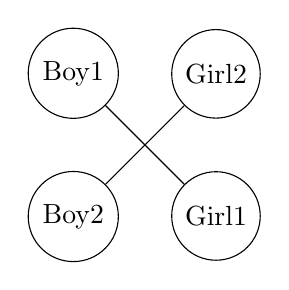
\begin{tikzpicture}
				\draw (0,1) node[anchor=south east,circle, draw]{Boy1} -- (1,0) node[anchor=north west, circle,draw]{Girl1};
				\draw (0,0) node[anchor=north east,circle, draw]{Boy2} -- (1,1) node[anchor=south west, circle,draw]{Girl2};
			\end{tikzpicture}
		\end{block}
		\pause
		\column{.30\textwidth}
		\begin{block}{Assignment Problems }
			\begin{figure}
				
\includegraphics[width=\linewidth]{tum_matching_small.png}
				% \caption{TUM Matching platform\footnote{\url{https://matching.in.tum.de/}}}
			\end{figure} 
		\end{block}
		\column{.30\textwidth}
		\pause
		\begin{block}{Kidney-Paired Donation}
			\begin{figure}
				
\includegraphics[width=\linewidth]{kidney_donation.jpg}
				% \caption{TUM Matching platform\footnote{\url{https://matching.in.tum.de/}}}
			\end{figure}
		\end{block}
		\end{columns} 
\end{frame}
% TODO
% Question about that the MATCHING SYSTEM is a Assignment Problems?????
% TODO
%     \footnote{David C. Parkes, Sven Seuken. Economics and Computation. Chapter 12: Matching Markets(pp. 291-293). 2017}


% Then I introduce the 3 Type of the maching Problems.
% The first one is the Two-Sided Matching. where there are two distinct groups of agents, and the problem is to match each agent on one side of the market with  an agent on the other side. 
% Like this graph here. I mean this two distinct group has the preference to each other. In word they can able to choose they matching, will have happy or sad feeling.
% Stable Marriage Problem belongs to this type. That we will disscuss later

% Second tyoe is Assignment Problems the matching, where there are items or resource and agents with preferences on resource, and  the problem is to assign a distinct resource to each agent.
% I would say the matching system and the this seminar is a good example here.
% To make a different distinglish them
% The chapitel in book or the exercise group are just item or recours
% They do not have preference. They just have to assigned to us. 
% Do you get the point? How to tell difference between the these two.

% The last type is Kidney-Paired Donation where patient-donor pairs arrive to the market, and the problem is to determine how to match pairs such that the donor in one pair is compatible with
%     the patient in another pair and vice versa, so that such a match enables two kidney transplants.
% There many factor that we have to consider about, blood type, when and where to do this operation(live transpant)
% And this is a big picture. We also have to befinit the most patient, to keep them health.

% In this handout and the presentation we will only talk about the Two-Sided Matching and Stable Marriage Problem, which is a case based on the this type of matching.

\begin{frame}{Matching in Graph}
	\begin{description}[leftmargin=!,labelwidth=\widthof{\bfseries strict preference order}]
		\item [\emph{Unweighted Graphs in Matching}]
	\end{description}
				\begin{itemize}
					\item  a vertex $v$ is matched in $M$: $M(v) \in V \setminus{v} : \{v, M(v)\} \in M$. 
					\item  Otherwise, $v$ is unmatched in $M$: $\{v, \emptyset\}$
				\end{itemize}
	\begin{description}[leftmargin=!,labelwidth=\widthof{\bfseries strict preference order}]
		\item [\emph{Bipartite Graph}] 
	\end{description}
	\begin{itemize}
		\item for every edge $(u,v)$:  $u$ $v$ in opposite subsets.
	\end{itemize}
\end{frame}

% TODO 
% {v, M(v)} or {u, v} are edges
%  M(v) is the matching of v, it could be a agent of the opperisite side

{
\setbeamercolor{background canvas}{bg=yellow!20}
\begin{frame}{Matching in Graph - Quiz1}
	Following are two graphs representing the matching between 2 sides. Which is a bipartite graph?
\begin{center}
    \begin{minipage}{.4\textwidth}
        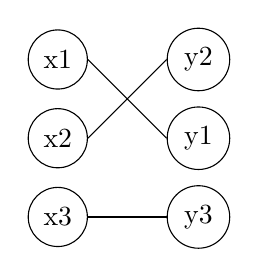
\begin{tikzpicture}
            \draw (0,2) node[anchor=east,circle, draw]{x1} -- (1,1) node[anchor=west, circle,draw]{y1};
            \draw (0,1) node[anchor=east,circle, draw]{x2} -- (1,2) node[anchor=west, circle,draw]{y2};
            \draw (0,0) node[anchor=east,circle, draw]{x3} -- (1,0) node[anchor=west, circle,draw]{y3};
        \end{tikzpicture} 
    \end{minipage}
    \begin{minipage}{.4\textwidth}
        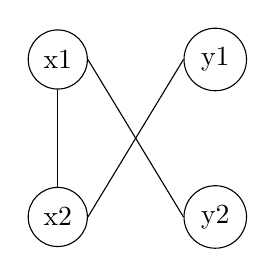
\begin{tikzpicture} 
            \node at (0,3) [circle, draw] (b1) {x1};
            \node at (0,1) [circle, draw] (b2) {x2};
            \node at (2,1) [circle, draw] (g1) {y2};
            \node at (2,3) [circle, draw] (g2) {y1};
            \draw (b1.east) -- (g1.west);
            \draw (b2.east) -- (g2.west);
            % \draw[red] (b1.south) -- (b2.north);
            \draw (b1.south) -- (b2.north);
        \end{tikzpicture}
    \end{minipage}
\end{center}
\vspace{1cm}
\end{frame}
}

% As I show in the last slide, the graph with boy and gril at the two side matching
% I think the group theroy is a fundematntal thing for our matching problem
% The graph to represent the two sided matching is th bipartite graph
% they have very simimar meaning - two sided or bipartit
% I have a quiz for you
% Just go with you natural intuition!!!

{
\setbeamercolor{background canvas}{bg=yellow!20}
\begin{frame}{Matching in Graph - Quiz1}
	Following are two graphs representing the matching between 2 sides. Which is a bipartite graph?
\begin{center}
    \begin{minipage}{.4\textwidth}
        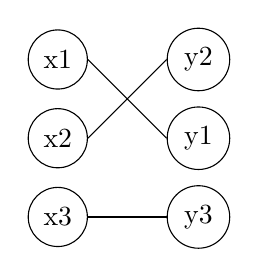
\begin{tikzpicture}
            \draw (0,2) node[anchor=east,circle, draw]{x1} -- (1,1) node[anchor=west, circle,draw]{y1};
            \draw (0,1) node[anchor=east,circle, draw]{x2} -- (1,2) node[anchor=west, circle,draw]{y2};
            \draw (0,0) node[anchor=east,circle, draw]{x3} -- (1,0) node[anchor=west, circle,draw]{y3};
        \end{tikzpicture} 
    \end{minipage}
    \begin{minipage}{.4\textwidth}
        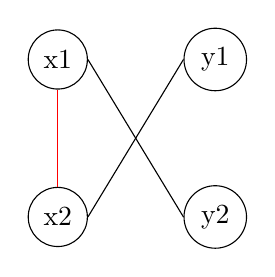
\begin{tikzpicture} 
            \node at (0,3) [circle, draw] (b1) {x1};
            \node at (0,1) [circle, draw] (b2) {x2};
            \node at (2,1) [circle, draw] (g1) {y2};
            \node at (2,3) [circle, draw] (g2) {y1};
            \draw (b1.east) -- (g1.west);
            \draw (b2.east) -- (g2.west);
            \draw[red] (b1.south) -- (b2.north);
            % \draw (b1.south) -- (b2.north);
        \end{tikzpicture}
		\end{minipage} \\
		\vspace{1cm}
		The left one is a bipartite graph. \\ The right one is not a bipartite graph.
\end{center}
\end{frame}
}
% Bacause the x1 x2 are connnected
% We have somehow a sequence of the node

\section{Stable Marriage Problem}
\begin{frame} 
	\tableofcontents[currentsection]
\end{frame}

\begin{frame}{Stable Marriage Problem}
	\begin{itemize}
		\item a set of men $X$ and a set of women $Y$.
		\item $M$ is set of marriages.
		\item $|X| = |Y| = N = |M|$.
		\item Only strict preference order.
		\item If $(x, y)\in M$, then $x = M(y)$ and $y = M(x)$.
		\item Or unmatched
	\end{itemize}
\end{frame}

%     The Stable Marriage Problem is a matching problem in graph theory first introduced
%     by Gale and Shapley\footnote{D. Gale and L. S. Shapley. College admissions and the stability of marriage. The American Mathematical Monthly. 1962}. An instance of this problem consists of two sets, a set of men
%     and a set of women. Each person specifies the order of all members of opposite sex. A
%     matching is stable if there is no pair where both man and woman prefer each other
%     to their current partner in the matching. The goal of this problem is to find a stable
%     matching for a given instance. Gale and Shapley proved that there always exists such a
%     matching for any instance. They also provided a polynomial algorithm for solving the
%     problem. 
%     \item[Stable Marriage Problem - Definition] An instance of the Stable Marriage Problem consists of a set of $n$
%     men and a set of $n$ women where each man and each woman provides a lineary strict preference order 
%     lists of all members of the opposite sex. Such lists are called preference lists.
%     Let $M$ be an one-to-one correspondence between the subset of men and the subset
%     of women, then $M$ is a marriage. If $(x, y) \in M$, called $(x, y)$
%     as a pair in $M$, means $x$ is married with $y$ in $M$ and $y$ is married with $x$ in $M$.
%     Furthermore, that a agent is unmatched in $M$ if he (or she) is not married
%     with any woman (or man) in $M$, otherwise this agent is matched in $M$. Let $M(x)$
%     denote the woman who is married with the man $x$ in $M$ and let $M(y)$ denote the man married
%     with the woman $y$ in $M$. Agents have only the strict preferences in this problem.


% Story: there are n men and n women, which
% are unmarried. Each has a preference list on
% the persons of the opposite sex
% • Does there exist and can we find a stable
% matching (stable marriage): a matching of
% men and women, such that there is no pair
% of a man and a woman who both prefer each
% other above their partner in the matching

\begin{frame}{Assumption: No Payments}
	\begin{figure}
		\tcbtp{
\includegraphics[width=.3\textwidth]{money_buy_love.png}}
		% \caption{TUM Matching platform\footnote{\url{https://matching.in.tum.de/}}}
	\end{figure}
\end{frame}
% it would be unusual, unethical, or against societal norms to use payments
% In our case we consider the preference order not with the payment, money!
% It is a assumptio also in the other matching

\begin{frame}{Assumption: Only Strict Preference Order}
	\pause
	\begin{figure}
		\tcbtp{
\includegraphics[width=.7\textwidth]{distracted_boyfriend.jpg}}
		% \caption{TUM Matching platform\footnote{\url{https://matching.in.tum.de/}}}
	\end{figure}
	\pause
	\begin{center}
		The strict preference order here: $y_{red} \succ_{x} y_{blue}$. \\ More specific $y_{red} \succ_{x} M(x)$.\\ 
		\pause
		Maybe this moment $y_{blue}$ prefer not to be matched with $x$ any more?
	\end{center}
\end{frame}
% This is a assumption in Stable Marriage Problem that we only have the  Strict Preference Order
% In word the man or woman have differenct order of reference on woman or man
% It's easy to undertstand this assumption, right?
% The feeling can not be exactly the same.

% Here is a example for that present this assumption very lively!
% 5 seconds to laugh
% How can I describe the strict preference order in this picture!

% Then we switch to the case that a agent can prefer not to be matched

\begin{frame}{Prefer to be Unmatched}
	\begin{itemize}
		\item $\emptyset \succ_{y_{red}} x$ 
		\item $x$ is \emph{unacceptable} for $y_{red}$
	\end{itemize}
\end{frame}
% An agent may prefer to be unmatched than matched with a particular agent on the other side.
% Preference $\emptyset \succ_y $ shows the intention of a woman $y$ who strictly prefers not to be matched than to be matched with man $x$.
% In this case, the man $x$ is said to be \emph{unacceptable} to the woman $y$. 

\begin{frame}{Blocking Pair and Stable Marriage}
	\begin{description}[leftmargin=!,labelwidth=\widthof{\bfseries Unstable Marriage}]
		\item [\emph{Blocking Pair}\footnote{Dan Gusfield, Robert W.Irving. The Stable Marriage Problem: Structure and Algorithms. Chapter 1: Elementary Concept and Result(pp. 6). The MIT Press, 1989}] if $(x, y) \notin M$ but:
	\end{description}
	\begin{itemize}[leftmargin=1em+4.5cm]
			\item $y$ prefers $x$ to $M(y)$ and
			\item $x$ prefers $y$ to $M(x)$
			\item If $\emptyset \succ_y M(y)$ for $y$, then $(y, \emptyset)$ form a blocking pair. Similar for $x$.
			% \item If $\emptyset \succ_x M(x)$ for $x$, then $(x, \emptyset)$ form a blocking pair. Similar for $y$.
	\end{itemize}
	\begin{description}[leftmargin=!,labelwidth=\widthof{\bfseries Unstable Marriage}]
		\item [\emph{Stable Marriage}\footnote{See footnote 2}] no blocking pair for $M$
		\item [\emph{Unstable Marriage}]  at least one blocking pair for $M$
	\end{description}
\end{frame}
% A blocking pair also exists when an agent prefers to be unmatched rather than assigned to his/her match.

{
\setbeamercolor{background canvas}{bg=yellow!20}
\begin{frame}{Blocking Pair and Stable Marriage - Quiz2}
	\textbf{Yes-No Questions}: Are the following statements true?
\begin{center}
	\begin{itemize}[leftmargin=1em+8mm]
    \item Man $x$ and woman $y$ form a blocking pair $(x, y)$ for matching $M$ if $M(x) \neq y$ and $M(x) \neq y$.\pause \\ \textcolor{red}{No} It should be corrected with $y \succ_x M(x)$ and $x \succ_y M(y)$
    \item A stable matching is one in which no pair of agents prefer each other over their respective matches. \pause \hspace{1cm} \textcolor{red}{Yes}
    % \item If $\emptyset \succ_y M(y)$ for a woman $y$, then $(y, \emptyset)$ form a blocking pair. \pause  \textcolor{red}{Yes}
\end{itemize}
\end{center}
\end{frame}
}

{
\setbeamercolor{background canvas}{bg=yellow!20}
\begin{frame}{Blocking Pair and Stable Marriage - Quiz2}
	\textbf{Last one}: Is this a unstable marriage regarding the context that we have talked about?
\begin{center}
	\begin{figure}
		
\includegraphics[width=.3\textwidth]{distracted_boyfriend.jpg}
		% \caption{TUM Matching platform\footnote{\url{https://matching.in.tum.de/}}}
	\end{figure}
	\pause
	I would say \textcolor{red}{yes}. We do have $y_{red} \succ_{x} M(x)$. \\
	\vfill
	\begin{description}[leftmargin=!,labelwidth=\widthof{\bfseries Blocking Pair}]
		\item [\emph{Blocking Pair}] if $(x, y) \notin M$ but:
	\end{description}
	\begin{itemize}[leftmargin=1em+2.5cm]
			\item \st{$y$ prefers $x$ to $M(y)$} and
			\item $x$ prefers $y$ to $M(x)$
			\item If $\emptyset \succ_y M(y)$ for a woman $y$, then $(y, \emptyset)$ form a blocking pair.
	\end{itemize}
	But I assume the $y_{blue}$ is $M(x)$ and at this moment she prefers not to be matched with $x$. Then a blocking pair $(y, \emptyset)$
\end{center}
\end{frame}
}
% welcome to our familiar example again!

% Because we knoe no thing about the girl in red.
% But it seems she has no interest on the boy
% Because she just go away

\begin{frame}{Gale–Shapley Deferred Acceptance Algorithm}
	\begin{theorem}
		[Gale–Shapley 1962] The Gale–Shapley algorithm guarantees to find a stable matching for \textbf{any} problem instance.
	\end{theorem} 
	\begin{center}
		\begin{figure}
			\tcbtp{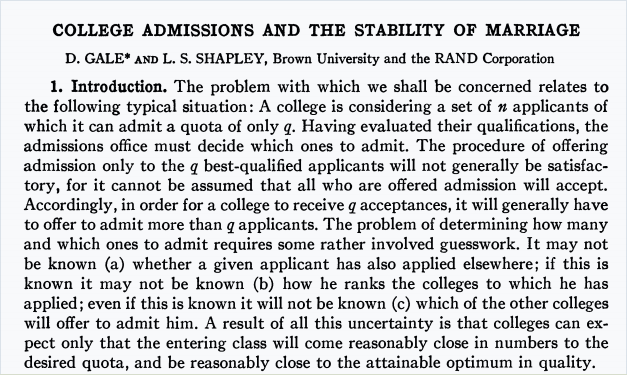
\includegraphics[width=.5\textwidth]{paper_algo.png}}
			% \caption{TUM Matching platform\footnote{\url{https://matching.in.tum.de/}}}
		\end{figure}
	\end{center}
\end{frame}

\begin{frame}{Gale–Shapley Deferred Acceptance Algorithm\footnote{D. Gale and L. S. Shapley. College admissions and the stability of marriage. The American Mathematical Monthly (pp.69:9–15). 1962}}
	\begin{center}
    \scalebox{0.95}{
    \begin{minipage}{0.95\linewidth}
			\tcbtp{\begin{algorithm}[H]
				\SetKwInOut{Input}{Input}
				\SetKwInOut{Output}{Output}
				\Input{a list of preference order}
				\Output{a stable marriage $M$}
				\underline{Initialize} $M$ to empty matching.\\
				\While{$x$ is unmatched and hasn't proposed to every woman}
					{
						$x$ proposes to the most-preferred woman $y$ to whom he has not yet propose\;
						\uIf{$y$ is unmatched}
						{
								add $(x, y)$ to $M$\; 
						}
						\uElseIf{$y$ prefers $x$ to current partner $x'$}
						{
								Replace $(x', y)$ with $(x, y)$ in $M$\;
						}
						\Else
						{
								$y$ rejects $x$\;
						}
					}
				\caption{GS DA Algorithm (men-proposing version)}
		\end{algorithm}}
    \end{minipage}%
    }
  \end{center}
\end{frame}
% Gale–Shapley Deferred Acceptance Algorithm (men-proposing version) 
% An intuitive method that guarantees to find a stable matching. That is very easy to understand
% even to act this algo in real life

% Each man proposes to her top-ranke woman (perhaps $\emptyset$). 
% Line 4 to 9 is nothing more than the y keep the most prefered proposal
% Each girl accepts the top-ranked proposal she receives (holding onto $\phi$ if this is preferred) 
% and rejects the other proposal .
% Each boy was rejected proposes to her top-ranked girl who has not yet rejected her proposal, or $\phi$ if this is now top-ranked amongst
% 	the remaining options.  
% The mechanism terminates when no new proposals are made. 
% At this point, each boy is matched with the girl (perhaps $\phi$) to whom she made her final proposal, and each girl is matched with the proposal she holds (perhaps $\phi$).

{
\setbeamercolor{background canvas}{bg=yellow!20}
\begin{frame}{Gale–Shapley D.A. Algorithm - Quiz3}
	Try to apply \textbf{Gale–Shapley Deferred Acceptance Algorithm} regarding the following preference list. There are three men and three women, with strict preference orders.
% \begin{center}
	\centerline{$y_2 \succ_{x_1} y_1 \succ_{x_1} y_3$ \;\;\;\;\;\;  $x_1 \succ_{y_1} x_3 \succ_{y_1} x_2$}  
	\centerline{$y_1 \succ_{x_2} y_3 \succ_{x_2} y_2$ \;\;\;\;\;\;  $x_3 \succ_{y_2} x_1 \succ_{y_2} x_2$}  
	\centerline{$y_1 \succ_{x_3} y_2 \succ_{x_3} y_3$ \;\;\;\;\;\;  $x_1 \succ_{y_3} x_3 \succ_{y_3} x_2$} 
	% \centerline{$x_1 \succ_{y_1} x_3 \succ_{y_1} x_2$}  
	% \centerline{$x_3 \succ_{y_2} x_1 \succ_{y_2} x_2$} 
	% \centerline{$x_1 \succ_{y_3} x_3 \succ_{y_3} x_2$} 
% \end{center}
\end{frame}
}
{
\setbeamercolor{background canvas}{bg=yellow!20}
\begin{frame}{Quiz3 - Step1}
	\centerline{$y_2 \succ_{x_1} y_1 \succ_{x_1} y_3$ \;\;\;\;\;\;  $x_1 \succ_{y_1} x_3 \succ_{y_1} x_2$}  
	\centerline{$y_1 \succ_{x_2} y_3 \succ_{x_2} y_2$ \;\;\;\;\;\;  $x_3 \succ_{y_2} x_1 \succ_{y_2} x_2$}  
	\centerline{$y_1 \succ_{x_3} y_2 \succ_{x_3} y_3$ \;\;\;\;\;\;  $x_1 \succ_{y_3} x_3 \succ_{y_3} x_2$} 
	\vfill
	\begin{center}
		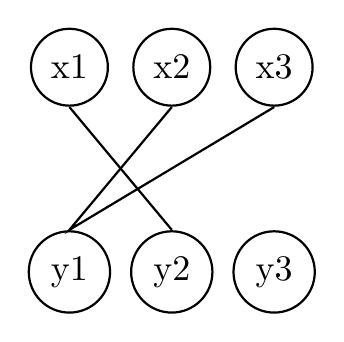
\begin{tikzpicture}[thick,scale=1.3, every node/.style={transform shape}]
			\node[circle, draw] at (0,-0.5) (y1){y1};
			\node[circle, draw] at (1,1.5) (x2){x2};
			\node[circle, draw] at (1,-0.5) (y2){y2};
			\node[circle, draw] at (0,1.5) (x1){x1};
			\node[circle, draw] at (2,1.5) (x3){x3};
			\node[circle, draw] at (2,-0.5) (y3){y3};
			\draw(y2.north)-- (x1.south);
			\draw (x3.south) -- (y1.north) -- (x2.south);
			% \draw (2,0) node[anchor=north, circle, draw]{y3};
		\end{tikzpicture} \\
		$y_1:$ $x_3$, $x_2$
	\end{center}
\end{frame}
}

{
\setbeamercolor{background canvas}{bg=yellow!20}
\begin{frame}{Quiz3 - Step1}
	\centerline{$y_2 \succ_{x_1} y_1 \succ_{x_1} y_3$ \;\;\;\;\;\;  $x_1 \succ_{y_1} x_3 \succ_{y_1} x_2$}  
	\centerline{$y_1 \succ_{x_2} y_3 \succ_{x_2} y_2$ \;\;\;\;\;\;  $x_3 \succ_{y_2} x_1 \succ_{y_2} x_2$}  
	\centerline{$y_1 \succ_{x_3} y_2 \succ_{x_3} y_3$ \;\;\;\;\;\;  $x_1 \succ_{y_3} x_3 \succ_{y_3} x_2$} 
	\vfill
	\begin{center}
		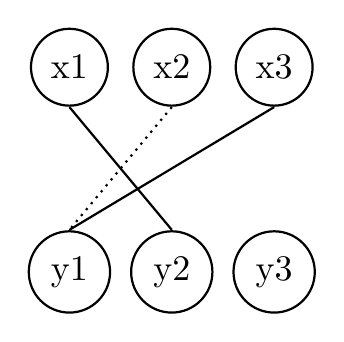
\begin{tikzpicture}[thick,scale=1.3, every node/.style={transform shape}]
			\node[circle, draw] at (0,-0.5) (y1){y1};
			\node[circle, draw] at (1,1.5) (x2){x2};
			\node[circle, draw] at (1,-0.5) (y2){y2};
			\node[circle, draw] at (0,1.5) (x1){x1};
			\node[circle, draw] at (2,1.5) (x3){x3};
			\node[circle, draw] at (2,-0.5) (y3){y3};
			\draw(y2.north)-- (x1.south);
			\draw (x3.south) -- (y1.north);
			\draw[dotted] (x2.south) -- (y1.north);
			% \draw (2,0) node[anchor=north, circle, draw]{y3};
		\end{tikzpicture} \\
		$y_1:$ \textcircled{$x_3$} \st{$x_2$} 
	\end{center}
\end{frame}
}
% \item In the first step, student $s1$ proposes to teacher $t2$, $s2$ to $t1$, and $s3$ to $t1$. 
% \item Teacher $t1$ has received two proposals and keeps $s3$, rejecting $s2$.
% Dach line is deleted


{
\setbeamercolor{background canvas}{bg=yellow!20}
\begin{frame}{Quiz3 - Step2}
	\centerline{$y_2 \succ_{x_1} y_1 \succ_{x_1} y_3$ \;\;\;\;\;\;  $x_1 \succ_{y_1} x_3 \succ_{y_1} x_2$}  
	\centerline{$y_1 \succ_{x_2} y_3 \succ_{x_2} y_2$ \;\;\;\;\;\;  $x_3 \succ_{y_2} x_1 \succ_{y_2} x_2$}  
	\centerline{$y_1 \succ_{x_3} y_2 \succ_{x_3} y_3$ \;\;\;\;\;\;  $x_1 \succ_{y_3} x_3 \succ_{y_3} x_2$}  
	\vfill
	\begin{center}
		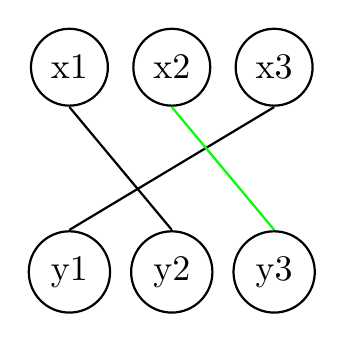
\begin{tikzpicture}[thick,scale=1.3, every node/.style={transform shape}]
			\node[circle, draw] at (0,-0.5) (y1){y1};
			\node[circle, draw] at (1,1.5) (x2){x2};
			\node[circle, draw] at (1,-0.5) (y2){y2};
			\node[circle, draw] at (0,1.5) (x1){x1};
			\node[circle, draw] at (2,1.5) (x3){x3};
			\node[circle, draw] at (2,-0.5) (y3){y3};
			\draw (y2.north) -- (x1.south);
			\draw (x3.south) -- (y1.north);
			\draw[green] (x2.south) -- (y3.north);
		\end{tikzpicture} 
		\\ $x_2:$ \st{$y_1$} \textcircled{$y_3$} $y_2$
	\end{center}
\end{frame}
}
% \item Since $s2$ is rejected, she proposes to her next most preferred teacher, $t3$ in the second step. 
% \item Now each teacher has exactly one proposal, no proposals are rejected, and the mechanism terminates. 
% \item The matching is $\{(s1,t2), (s2,t3), (s3,t1)\}$, which is the stable matching.
{
\setbeamercolor{background canvas}{bg=yellow!20}
\begin{frame}{Quiz3 - Step2}
	\centerline{$y_2 \succ_{x_1} y_1 \succ_{x_1} y_3$ \;\;\;\;\;\;  $x_1 \succ_{y_1} x_3 \succ_{y_1} x_2$}  
	\centerline{$y_1 \succ_{x_2} y_3 \succ_{x_2} y_2$ \;\;\;\;\;\;  $x_3 \succ_{y_2} x_1 \succ_{y_2} x_2$}  
	\centerline{$y_1 \succ_{x_3} y_2 \succ_{x_3} y_3$ \;\;\;\;\;\;  $x_1 \succ_{y_3} x_3 \succ_{y_3} x_2$}  
	\vfill
	\begin{center}
		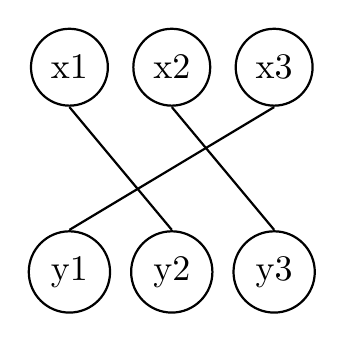
\begin{tikzpicture}[thick,scale=1.3, every node/.style={transform shape}]
			\node[circle, draw] at (0,-0.5) (y1){y1};
			\node[circle, draw] at (1,1.5) (x2){x2};
			\node[circle, draw] at (1,-0.5) (y2){y2};
			\node[circle, draw] at (0,1.5) (x1){x1};
			\node[circle, draw] at (2,1.5) (x3){x3};
			\node[circle, draw] at (2,-0.5) (y3){y3};
			\draw (y2.north) -- (x1.south);
			\draw (x3.south) -- (y1.north);
			\draw (x2.south) -- (y3.north);
		\end{tikzpicture} 
		\\ $x_2:$ \st{$y_1$} \textcircled{$y_3$} $y_2$  
		\\ Stable now!
	\end{center}
\end{frame}
}

\begin{frame}{Proof of Correctness: Termination}
	\begin{description}[leftmargin=!,labelwidth=\widthof{\bfseries Observation 1}]
		\item [Observation 1] Man proposes to woman in decreasing order of preference.
		\item [Observation 2] Once a woman is matched, she never becomes unmatched. 
		\item [Observation 3] No agent proposes to another agent more than once,
	\end{description}
	\begin{theorem}
    The algorithm terminates in at most $N ^2$ iterations
\end{theorem} 
\end{frame}
% Once a woman is matched, she stays matched (her partner can change).
% When the partner of a woman changes, this is to a more preferable partner for her: at most n – 1 times.

\begin{frame}{Proof of Correctness: Termination}
	\begin{theorem}
    The algorithm terminates in at most $N ^2$ iterations
\end{theorem}   
\begin{proof}
    \begin{itemize}
			\item Each iteration, $x$ proposes to $y$ to whom he has not proposed	before
			\item Proposal can be rejected.
			\item $|X| = |Y| = N$.
			\item $N * N$ possible proposals.
		\end{itemize}
\end{proof}
\begin{center}
	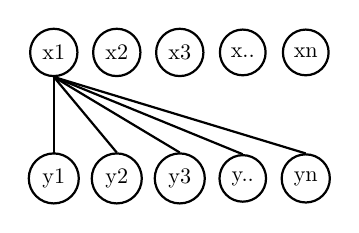
\begin{tikzpicture}[thick,scale=0.8, every node/.style={transform shape}]
		\node[circle, draw] at (0,-0.5) (y1){y1};
		\node[circle, draw] at (1,1.5)  (x2){x2};
		\node[circle, draw] at (1,-0.5) (y2){y2};
		\node[circle, draw] at (0,1.5)  (x1){x1};
		\node[circle, draw] at (2,1.5)  (x3){x3};
		\node[circle, draw] at (2,-0.5) (y3){y3};
		\node[circle, draw] at (3,-0.5) (y){y..};
		\node[circle, draw] at (3,1.5)  (x){x..};
		\node[circle, draw] at (4,1.5)  (xn){xn};
		\node[circle, draw] at (4,-0.5) (yn){yn};
		\draw (y2.north) -- (x1.south);
		\draw (y1.north) -- (x1.south);
		\draw (y3.north) -- (x1.south);
		\draw (y.north) -- (x1.south);
		\draw (yn.north) -- (x1.south);

	\end{tikzpicture} 
\end{center}
% (Can be tighten a bit to $N(N ‐ 1) + 1$ iterations.)
\end{frame}

% N(N ‐ 1) + 1
%     This just puts an upper-bound on the number of rounds that can take place
%     in this algorithm. Notice that at every round except the last round, a man crosses
%     a woman off his list. And since every man gets married, he can cross off no more
%     than $(N - 1)$ women. So there are no more than $N * (N - 1)$ cross-offs and thus no
%     more than $N*(N - 1) + 1$ rounds.

\begin{frame}{Proof of Correctness: Matching}
\begin{theorem}
    Everybody gets married
\end{theorem} 
\begin{proof}
	\begin{itemize}
		\item Once a woman is matched, she never becomes unmatched.
		\item Man is always rejected then be unmatched.
		\item Assume there exists a man that is not machted, then also a woman unmatched.
		\item Proved using a contradiction.
	\end{itemize}
\end{proof}
\end{frame}

% \begin{prf}
%     First note that once a woamn is proposed to, she is engaged to be married
%     and will never lose that. She can only trade up to better man for matching on her list. 

%     And since each man was ranked by every woman, the only way that a man will not be
%     married is if she is rejected by every woman.

%     Assume there exists a man that is not married, then there also must be woman who is unmarried. But this unmarried
%     man must have been proposed to at one point by the unmarried woman, thus he
%     must be married. Contradiction, so everybody gets married.



\begin{frame}{Proof of Correctness: Sability}
	\begin{theorem}
		The algorithm produces a stable matching.
	\end{theorem} 
	\begin{proof}
		\begin{itemize}
			\item Assume there exists a blocking pair $(x, y)$. So $x \succ_y M(y)$ and $y \succ_x M(x)$
			\item $x$ must have proposed to $y$ and $y$ rejected $x$.
			\item $y$ only reject $x$, when $M(y) \succ_y x$
			\item Proved using a contradiction.
		\end{itemize}
	\end{proof}
	\end{frame}
% We have seen that this contradiction is a powerful tool for proving
% So we also recap that and try to continue to apply that is this case

%     Assume the opposite, that the matching is not stable. So there must be at least one
% blocking pair, $(x, y)$. Suppose $x$ married $y'$ (who he likes less than $y$) and that
% $y$ married $x'$ (who she likes less than $x$). 
% That means $x$ must have proposed to $y$ at one point and she rejected him. But the only way that $y$ would reject $x$ is if
% she had a proposal from somebody she liked better. But women can only trade up
% from round to round, which means she must like $x'$ better than $y$. Contradiction,
% so the matching must be stable.




% Do all executions of Gale–Shapley lead to the same stable matching?
% A. No, because the algorithm is nondeterministic.
% B. No, because an instance can have several stable matchings.
% C. Yes, because each instance has a unique stable matching.
% D. Yes, even though an instance can have several stable matchings

% and the algorithm is nondeterministic.





% Herr kopplerungman
% TODO Martin




\begin{frame} 
	\tableofcontents[currentsection]
\end{frame}

\section{Context}
\begin{frame} 
	\tableofcontents[currentsection]
\end{frame}

\begin{frame}{2012 Nobel Prize in Economics}
	\begin{description}
		\item [Lloyd Shapley.] Stable matching theory and Gale–Shapley algorithm.
	\end{description}
	\begin{figure}
		\tcbtp{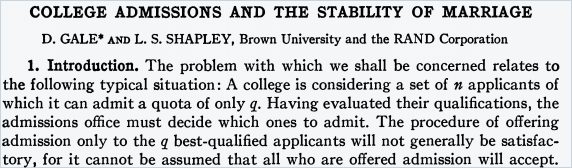
\includegraphics[width=.5\linewidth]{paper.png}}
	\end{figure} 
	\begin{description}
		\item [Alvin Roth.] Applied Gale–Shapley to matching med-school students with
		hospitals, students with schools, and organ donors with patients.
	\end{description}
	\begin{figure}
		\tcbtp{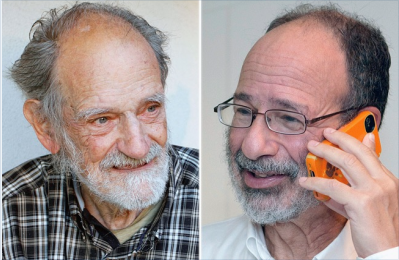
\includegraphics[width=.25\linewidth]{shapley_and_roth}}
		\caption{Lloyd Shapley(left) and Alvin Roth(right)}
	\end{figure} 
\end{frame}
	
\begin{frame}{Application: Matching Residents to Hospitals}
	\begin{itemize}
		\item National Resident Matching Program (NRMP)\footnote{\url{https://en.wikipedia.org/wiki/National_Resident_Matching_Program}}.
		\item Original use just after WWII.
		\item Match med-school students to hospitals.
		\item Men $\thickapprox$ hospitals, Women $\thickapprox$ med school residents. But not same!
		\item Also called \textbf{The MATCH}.
	\end{itemize}
\end{frame}
% eariler than the computer use
% But they are not complectly same 
% Hospitals/Residents we lost the assumption that we made for marriage. Student and hospital are not same number
% In face these two are very complicated, and both been researched decades

% FUNNY is this organiztion using the program is also called the match
% as I always keep repeating the match this. 
% It can be our matching system, our seminar mathcing, marriage matching, and this organization
% I hope I can lever a little memory. So next time you use matching system. 
% You can say AHA that the matching that I have seen in the seminar.
% A chinese guy have presented that in my seminar
% The AHA monent can increse our achinvement right!
% You will also be prove of youself at that AHA moment, you can say that you know the terminology and the algorithmun about that .

% Its mission medical school students and graduates into residency and fellowship training programs.
% assignment of medical students to
% hospitals (for internships)
% – Students list hospitals in order of preference
% – Hospitals list students in order of preference


\section{Summary}
\begin{frame} 
	\tableofcontents[currentsection]
\end{frame}

\begin{frame}
\frametitle{Summary}

% \begin{itemize}
% 	\item Item 1
% 	\item Item 2
% 	\item Item 3
% \end{itemize}
% \vfill
% Question?
\begin{columns}[t]
\column{.25\textwidth}
\begin{block}{\small{Stable Marriage Problem}}
	\begin{itemize}
		\item \small{$|X| = |Y| = N = |M|$}
		\item \small{$(x, y)\in M \equiv x = M(y) \land y = M(x)$.}
	\end{itemize}

\includegraphics[width=.3\linewidth]{money_buy_love.png}

\includegraphics[width=.5\linewidth]{distracted_boyfriend.jpg}
\end{block}

\column{.25\textwidth}
\begin{block}{\small{Blocking Pair}}
	\begin{itemize}
			\item \small{$x \succ_y M(y)$}
			\item \small{$y \succ_x M(x)$}
			\item \small{$\emptyset \succ_y M(y) \Rightarrow (y, \emptyset)$}
	\end{itemize}
\end{block}
\begin{block}{\small{Stable Marriage}}
	 \small{No blocking pair for $M$.}
\end{block}

\column{.5\textwidth}
\begin{block}{\small{GS DA Algorithm -- $O(n^2)$}}
	\begin{center}
    \scalebox{.8}{
    \begin{minipage}{1.2\linewidth}
			\tcbtp{\begin{algorithm}[H]
				% \SetKwInOut{Input}{Input}
				% \SetKwInOut{Output}{Output}
				% \Input{a list of preference order}
				% \Output{a stable marriage $M$}
				\underline{Initialize} \small{$M$ to empty matching.}\\
				\While{\small{$x$ is unmatched and hasn't proposed to every woman}}
					{
						$x$ proposes to the most-preferred and not proposed woman $y$\;
						\uIf{$y$ is unmatched}
						{
								add $(x, y)$ to $M$\; 
						}
						\uElseIf{$y$ prefers $x$ to current partner $x'$}
						{
								Replace $(x', y)$ with $(x, y)$ in $M$\;
						}
						\Else
						{
								$y$ rejects $x$\;
						}
					}
				% \caption{GS DA Algorithm (men-proposing version)}
		\end{algorithm}}
    \end{minipage}%
    }
	\end{center}
\end{block}
\end{columns}
\pause
\begin{center}
	Any Questions?
\end{center}
\end{frame}

\end{document}